% This file was created with tikzplotlib v0.10.1.post5.
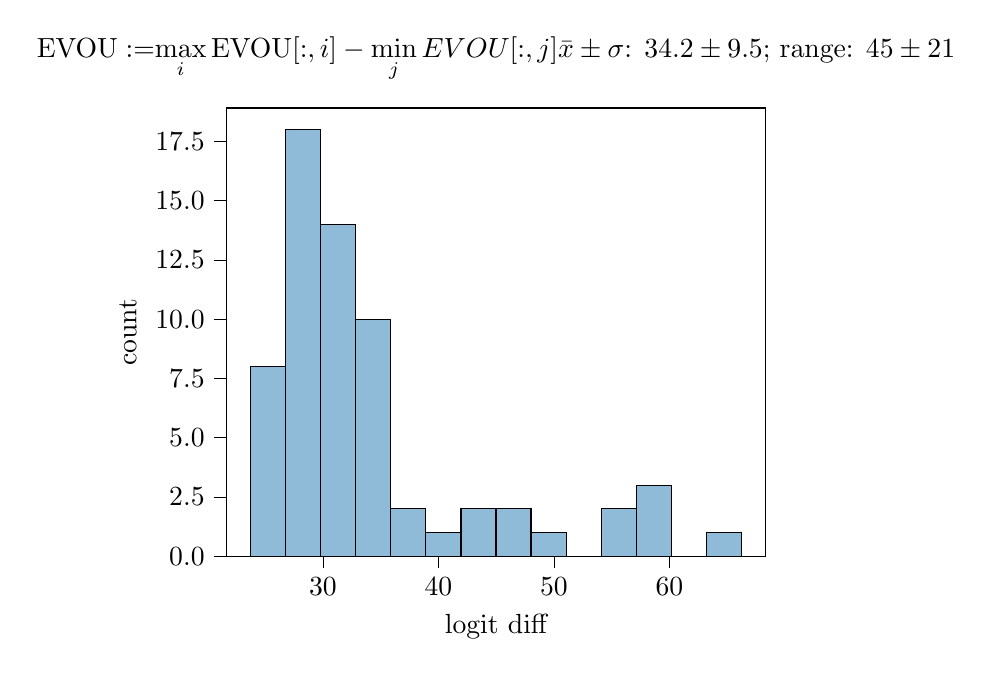
\begin{tikzpicture}

\definecolor{darkgray176}{RGB}{176,176,176}
\definecolor{steelblue31119180}{RGB}{31,119,180}

\begin{axis}[
tick align=outside,
tick pos=left,
title={\(\displaystyle \mathrm{EVOU} := \WE \WV \WO\WU \)\\
\(\displaystyle \max_i\mathrm{EVOU}[:,i] - \min_jEVOU[:,j]\)\\
\(\displaystyle \bar{x}\pm\sigma\): \(\displaystyle 34.2 \pm 9.5\); range: \(\displaystyle 45 \pm 21\)},
x grid style={darkgray176},
xlabel={logit diff},
xmin=21.6173468589783, xmax=68.352721118927,
xtick style={color=black},
xtick={20,30,40,50,60,70},
xticklabels={
  \(\displaystyle {20}\),
  \(\displaystyle {30}\),
  \(\displaystyle {40}\),
  \(\displaystyle {50}\),
  \(\displaystyle {60}\),
  \(\displaystyle {70}\)
},
y grid style={darkgray176},
ylabel={count},
ymin=0, ymax=18.9,
ytick style={color=black},
ytick={0,2.5,5,7.5,10,12.5,15,17.5,20},
yticklabels={
  \(\displaystyle {0.0}\),
  \(\displaystyle {2.5}\),
  \(\displaystyle {5.0}\),
  \(\displaystyle {7.5}\),
  \(\displaystyle {10.0}\),
  \(\displaystyle {12.5}\),
  \(\displaystyle {15.0}\),
  \(\displaystyle {17.5}\),
  \(\displaystyle {20.0}\)
}
]
\draw[draw=black,fill=steelblue31119180,fill opacity=0.5] (axis cs:23.7416820526123,0) rectangle (axis cs:26.7764466149466,8);
\draw[draw=black,fill=steelblue31119180,fill opacity=0.5] (axis cs:26.7764466149466,0) rectangle (axis cs:29.811211177281,18);
\draw[draw=black,fill=steelblue31119180,fill opacity=0.5] (axis cs:29.811211177281,0) rectangle (axis cs:32.8459757396153,14);
\draw[draw=black,fill=steelblue31119180,fill opacity=0.5] (axis cs:32.8459757396153,0) rectangle (axis cs:35.8807403019496,10);
\draw[draw=black,fill=steelblue31119180,fill opacity=0.5] (axis cs:35.8807403019496,0) rectangle (axis cs:38.915504864284,2);
\draw[draw=black,fill=steelblue31119180,fill opacity=0.5] (axis cs:38.915504864284,0) rectangle (axis cs:41.9502694266183,1);
\draw[draw=black,fill=steelblue31119180,fill opacity=0.5] (axis cs:41.9502694266183,0) rectangle (axis cs:44.9850339889526,2);
\draw[draw=black,fill=steelblue31119180,fill opacity=0.5] (axis cs:44.9850339889526,0) rectangle (axis cs:48.019798551287,2);
\draw[draw=black,fill=steelblue31119180,fill opacity=0.5] (axis cs:48.019798551287,0) rectangle (axis cs:51.0545631136213,1);
\draw[draw=black,fill=steelblue31119180,fill opacity=0.5] (axis cs:51.0545631136213,0) rectangle (axis cs:54.0893276759556,0);
\draw[draw=black,fill=steelblue31119180,fill opacity=0.5] (axis cs:54.0893276759556,0) rectangle (axis cs:57.12409223829,2);
\draw[draw=black,fill=steelblue31119180,fill opacity=0.5] (axis cs:57.12409223829,0) rectangle (axis cs:60.1588568006243,3);
\draw[draw=black,fill=steelblue31119180,fill opacity=0.5] (axis cs:60.1588568006243,0) rectangle (axis cs:63.1936213629586,0);
\draw[draw=black,fill=steelblue31119180,fill opacity=0.5] (axis cs:63.1936213629586,0) rectangle (axis cs:66.228385925293,1);
\end{axis}

\end{tikzpicture}
